% Document type, font size, margin
\documentclass[11pt]{article}

% Double spacing and indentation
\usepackage{setspace}
\doublespacing
\setlength{\parindent}{0pt}

\usepackage{csquotes}

% Package required for biber/biblatex
\usepackage[
    backend=biber,
    style=authoryear-icomp,
    sortlocale=de_DE,
    natbib=true,
    url=false, 
    doi=true,
    eprint=false
]{biblatex}
\addbibresource{mybib.bib}

% Set font to Arial (Tom Adcock)
% \usepackage{fontspec}
% \setmainfont[
% BoldFont=Arial Bold.ttf,
% ItalicFont=Arial Italic.ttf,
% BoldItalicFont=Arial Bold Italic.ttf
% ]{Arial.ttf}

% CHANGING FONT TO BE COMPATIBLE WITH PDFLATEX COMPILER
\usepackage[T1]{fontenc}
\renewcommand*\familydefault{\sfdefault}

% If you have Arial installed on your system, you can use it with pdflatex
\renewcommand{\rmdefault}{phv} % Helvetica as the main font
\renewcommand{\sfdefault}{phv} % Helvetica as the sans-serif font

% Given by "Example Project"
\usepackage[english]{babel}
\usepackage[a4paper,top=2cm,bottom=2cm,left=3cm,right=3cm,marginparwidth=1.75cm]{geometry}

% Useful packages
\usepackage{amsmath}
\usepackage{amssymb}
\usepackage{graphicx}
\usepackage{tabularx}
\usepackage{subcaption}
\usepackage[justification=centering]{caption}
\usepackage{multicol}
\usepackage{fancyhdr} % Include the package for custom headers and footers
\usepackage{lipsum}   % Provides sample text. Remove this in your actual document
\usepackage{hyperref}
\usepackage{parskip}
\usepackage{fancyvrb}
\usepackage{titlesec}
\usepackage{bm}
\usepackage{pdflscape}


\setlength\parindent{20pt}

% Headers and footers
\pagestyle{fancy}     % Set the page style to fancy to apply your custom headers and footers
\fancyhf{}            % Clear all header and footer fields to start fresh
% Default header and footer settings
\fancyhead{}          % Clear all header fields
\fancyhead[L]{\leftmark} % "\leftmark" will display the current section name
\fancyfoot{}          % Clear all footer fields
\fancyfoot[C]{\thepage}  % Page number at the bottom center
\setlength{\headheight}{15pt}
\addtolength{\topmargin}{-1.6pt}  % Line width for the header rule
\renewcommand{\footrulewidth}{0pt}    % No line for the footer

% Define the null header
\fancypagestyle{nullheader}{
  \fancyhf{} % Clear headers and footers
  \renewcommand{\headrulewidth}{0pt} % No line in the header
  \renewcommand{\footrulewidth}{0pt} % No line in the footer
}

% Text that was with the HAZOP analysis
\renewcommand{\familydefault}{\sfdefault}
\usepackage{graphicx}
\usepackage{float}
\usepackage{fancyhdr}
\usepackage{multirow} 
\usepackage{lipsum}
\usepackage{array} % required for text wrapping in tables
\usepackage{lscape} 
\usepackage[table,xcdraw]{xcolor}

% Start of the document
\begin{document}
% Apply the cover page style for the cover page
\thispagestyle{nullheader}

\vspace*{2cm}
\begin{center}
\huge{\textbf{B3 Group Design Project}}\\
\huge{\textbf{Cultured Beef Production}}\\
\begin{figure}[h]
    \centering
    
\includegraphics[width=0.45\textwidth]{y0-oxford.jpg}
    \hfill
\end{figure}
\vspace*{-1cm}
{\Large Mikhail Agureev, Eunsoo Chang, William Hough, Tracey Saber}\\ % Enlarge names slightly
{\Large University of Oxford}\\ % Add some space after the university name
\vspace*{1cm}
{\large Department of Engineering Science}\\ % Separate department
{\large supervised by J. Kwan, N. Hankins, B. Nie, P. Mouthuy}\\[0.5cm] % Separate supervision line
\vspace*{0.5cm}
{\large Trinity Term 2024}

\thispagestyle{empty} % Remove page number
\end{center}
\clearpage % End of the cover page

\thispagestyle{nullheader}


\tableofcontents
\clearpage % Starts a new page after the table of contents

\thispagestyle{nullheader}
\newpage

\textbf{MAINLY TALK ABOUT WHY YOUR CHOICE LED TO A BETTER ACHIEVEMENT OF THE DESIGN OBJECTIVES.}\\

The generic structure of a technical report:

1. Introduction: Provide context, motivation, and background information

What is the big-picture problem? Why is it a problem? Who cares?

What have others done to solve the problem? What is still left to do? What did you do?

2. Methods: Explain what you did
Provide enough detail for someone else to reproduce your results.

For each aspect, the level of detail should be commensurate with the level of novelty.

3. Results: Show and explain what you found.
Provide figures and other qualitative and quantitative evidence for your conclusions.

Explain and interpret what you are showing. Not "What does the data look like?", but "What does the data mean?"

4. Discussion: Consider the implications and limitations of your results

5. Conclusions: Connect your results with the original problem.

What have you actually achieved here? What should be done next?\\

Tip 1. Emphasise results, interpretation, and discussion.

Tip 2. Technical writing needs to be precise, concise, objective, careful

Tip 3. Every sentence must: (i) make a point (ii) form a logical link between the previous sentence and the next\\
\clearpage % Starts a new page after the table of contents

\fancyhead[L]{}
\fancyhead[R]{INTRODUCTION - WILL HOUGH}
\newpage
\section{Abstract}

\subsection*{Introduction}

It’s becoming clear that the livestock farming sector is one of the main contributors to the world’s water depletion, land use, biodiversity loss and greenhouse gas emissions. Over a third of the world’s crop calories are used as animal feed, and only a third of those feed calories end up contributing to the human diet. [https://iopscience.iop.org/article/10.1088/1748-9326/8/3/034015] With trends in global consumption and production of meat growing, the impacts of livestock farming are set to grow.
Alternative protein developments aim to substantially reduce the impact of feeding the human and domesticated animal population of the world by substituting the billions of animals grown and slaughtered every year with an alternative. There are significant developments in the plant-based, microbial, and fermented protein research, but we focus on evaluating the viability of directly substituting reared and slaughtered cattle with commercially cultured beef. 

% \begin{figure}[h]
%     \centering
%     
\includegraphics[width=0.75\textwidth]{will/example-image.jpg}
%     \hfill
%     \caption{An example image \citet{E-Cannon2022}}
%     \label{fig:example-image}
% \end{figure}

\subsection*{Summary}

Whilst shifting crop use away from animal feed could feed an additional 4 billion people and reduce global Green House Gas emissions by about a tenth, our venture proposal wouldn’t be profitable in today’s political and economic climate. [https://iopscience.iop.org/article/10.1088/1748-9326/8/3/034015] [https://www.sciencedirect.com/science/article/pii/S0377840111001933 MAKE SURE TO ACCOUNT FOR INCREASE IN CROP CONSUMPTION]
Unless commissioned by a special interested party – the outgoings and capital cost, along with risk associated with such a new, volatile and saturated market – mean that the proposal is unlikely to work better than other protein alternatives. If policies were introduced that reduced the subsidies on traditionally farmed meat and moved them to cultured meat, then our proposal might gain more traction to feed demand as our prices ease. [https://www.oxfordmartin.ox.ac.uk/blog/meat-and-dairy-gobble-up-farming-subsidies/]

% Example equation \ref{eq:example-equation}.

% \begin{equation}
%     beef_{moo} = fear^{10}
%     \label{eq:example-equation}
% \end{equation}

% Example list:

% \begin{itemize}
%     \item \(\bm{X} \in \mathbb{R}^{n \times p}\), a matrix containing the scrutinised data-points $\bm{x} \in \mathbb{R}^{p}$ from each sample,
%     \item \textit{regression\textunderscore targets}, known as $\bm{\bar{y}}\in \mathbb{R}^n$, is a vector containing the regression targets for the samples (individually known as $\Bar{y}$), and
%     \item \textit{class\textunderscore labels} $\in \{1,\dots,p\}$ which keeps track of which Gaussian each sample came from (a target for classification).
% \end{itemize}

% Example table \ref{table:1}

% \begin{table}[!ht] % the [h] forces the table to be "here". This is quite a short document so LaTeX struggles to find a nice arrangement for the floats! Not normally needed
%     \begin{center}
    
%         \begin{tabular}{|l|c|c|} 
%             \hline
%             \textbf{learning\_rate} & \textbf{mse\_train} & \textbf{mse\_val} \\ 
%             \hline
%             1e-05&1.1254&1.1747\\
%             \hline
%             0.0001&0.31296&0.3012\\
%             \hline
%             0.001&0.095492&0.088045\\
%             \hline
%             0.01&0.046835&0.052905 \\
%             \hline
%             0.1&0.046534&0.052771\\
%             \hline
%             1&NaN&NaN \\
%             \hline
%         \end{tabular}
%         \caption{Table of Mean Squared Difference from different learning rates.}
%         \label{table:1}
            
%     \end{center}
% \end{table}

% Example aligned equation:

% \begin{align*}
%     \mathcal{L}_c &= -ylog(\bar{y}) - (1-y)log(1-\bar{y})\\
%     &= ylog(1+e^{-\bm{\hat{x}^T\theta}})-(1-y)log(\frac{e^{-\bm{\hat{x}^T\theta}}}{1+e^{-\bm{\hat{x}^T\theta}}})\\
%     &=(y-y)log(1+e^{-\bm{\hat{x}^T\theta}})-(1-y)log(e^{-\bm{\hat{x}^T\theta}})+log(1+e^{-\bm{\hat{x}^T\theta}})\\
%     &=(1-y)\bm{\hat{x}^T\theta}+log(1+e^{-\bm{\hat{x}^T\theta}})\\
%     \Delta_{\bm{\theta}}\mathcal{L}_c &=(1-y)\bm{\hat{x}}-\frac{e^{-\bm{\hat{x}^T\theta}}}{1+e^{-\bm{\hat{x}^T\theta}}}\bm{\hat{x}}\\
%     &=(1-y)\bm{\hat{x}}-(1-\bar{y})\bm{\hat{x}}\\
%     &=\bm{\hat{x}}(\bar{y}-y)
% \end{align*}

% END OF TEMPLATE

\fancyhead[L]{}
\fancyhead[R]{MEDIUM - TRACEY SABER}
\input{tracey/T1-Medium}

\fancyhead[L]{}
\fancyhead[R]{PROLIFERATION SEED - TRACEY SABER}
\input{tracey/T2-Proliferation}

\fancyhead[L]{}
\fancyhead[R]{CONTROL SYSTEMS - EUNSOO CHANG}
\newpage
\section{Control systems}
\vspace{-3mm}
\subsection{Introduction}
\vspace{-3mm}

% 4 pages given, 8 sections in total.
% Each section should be roughly 1/2 page long.

% - (I) What is a bioreactor control system?

Homeostasis, defined as the internal regulatory functions of the body to maintain certain conditions constant~\citep{E-Guyton2006, E-Aging2022}, is extremely crucial to living organisms. For example, for humans, the blood pH outside the range between 7.35 and 7.45 can cause death \cite{E-Donaldson2013}. In addition to its significance in maintaining an existing life, homeostasis has great importance in creating a new life: Mammalian cell culture.

In a bioreactor, homeostasis can be achieved by solving the classical problem of tracking the reference signal $r(t)$ in control theory, as shown in Figure \ref{figure:E-1-1-control-system}. A thoroughly designed bioreactor and its constituent control systems will lead to better achievement of the design objectives, which are: (i) How can one achieve the production rate of 100 kg/month? (ii) How can one produce a better quality of meat?

The design of the control system mainly answers the latter question. The former question is rather answered through the overall process diagram, number and sizes of bioreactors, mass inflows and outflows, so will not be tackled in this chapter. Bioreactor control, however, addresses the formation and maintenance of the optimal environment to produce the best quality of meat. Thus, in this chapter, the design of temperature (T), dissolved oxygen (DO) and acidity (pH) control systems are discussed.

\begin{figure}[h]
    \centering
    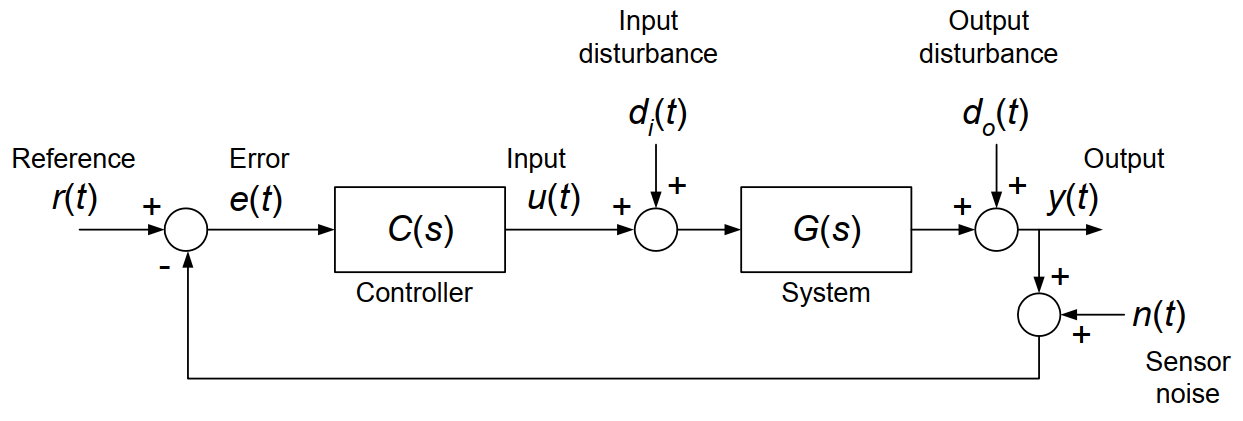
\includegraphics[width=0.75\textwidth]{eunsoo/E-1-1-control-system.png}
    \hfill
    \caption{A schematic of a negative feedback control system \citet{E-Cannon2022}}
    \label{figure:E-1-1-control-system}
\end{figure}

\vspace{-10mm}
\subsection{Temperature control}
\vspace{-3mm}
\subsubsection{Introduction}

% - (I) why consider control systems for temperature?

The body temperature of beef cattle should be maintained at $39.6 \pm 0.1 ^{\circ} C$ \cite{E-Gaughan2014}. To do so, different physical setups of the heat exchanger around the bioreactor will be compared to find the optimal one. Differential equations will be constructed to derive the plant transfer function. Design criteria will be posed with appropriate justification. Different control strategies will be compared to find the optimal one. The design criteria introduced will be used to find control parameters. MATLAB simulations will be used to confirm the validity of the step and impulse responses.

\subsubsection{Methods}

% - (M1) the physical structure of the temperature control system and justification

Various types of heat exchangers used to control the heat in and out of the bioreactor are shown in Figure \ref{figure:E-1-2-heat-exchangers}. The best design choice is (a), the jacketed bioreactor. The logic is as follows: (c) and (d) have the heat exchange inside the bioreactor, causing an intervention in the rotational pathway of the impeller used to stir the meat, and thus adding unnecessary complexity to the design to avoid this; (e) involves taking the meat out of the bioreactor, which firstly may harm the meat cells by pumping and pressurising them above the maximum stress that they they can resist, and secondly has a potential issue of fouling in the pump. One is now left with (a) and (b), but for better heat transfer it is more efficient for the working fluid to cover the entire bioreactor, and for more evenly distributed heat transfer it is better if the inlet and the outlet temperatures of the heat exchanger do not vastly differ. Hence, (a) is the best option.

\begin{figure}[h]
    \centering
    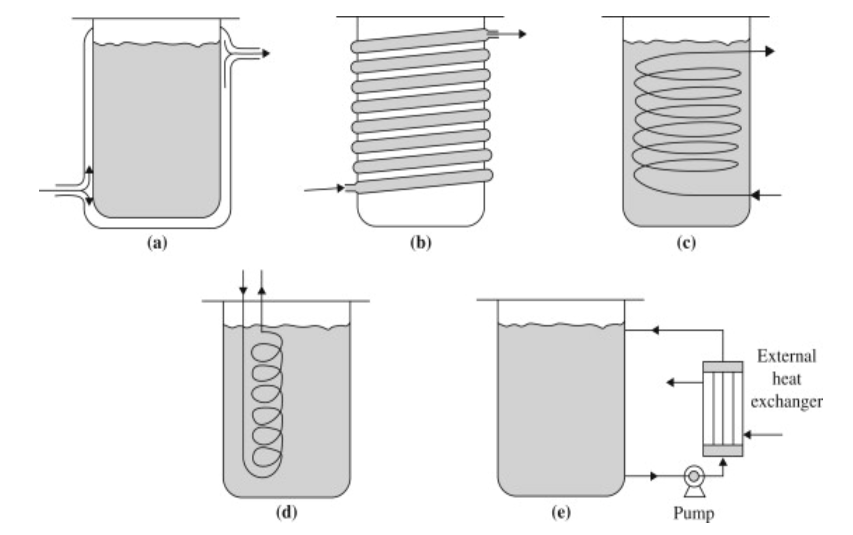
\includegraphics[width=0.5\textwidth]{eunsoo/E-1-2-heat-exchangers.png}
    \hfill
    \caption{Heat exchanger configurations for a bioreactor \cite{E-Doran2013}}
    \label{figure:E-1-2-heat-exchangers}
\end{figure}

\vspace{-5mm}
Theoretically, the heat exchanger's working fluid temperature $T_{fluid}$ controls the bioreactor's internal temperature $T$. Practically, the observer is implemented using a temperature sensor, and the controller is implemented digitally using a computer system, as shown in Figure \ref{figure:E-1-3-digital-control-system}.

\begin{figure}[h]
    \centering
    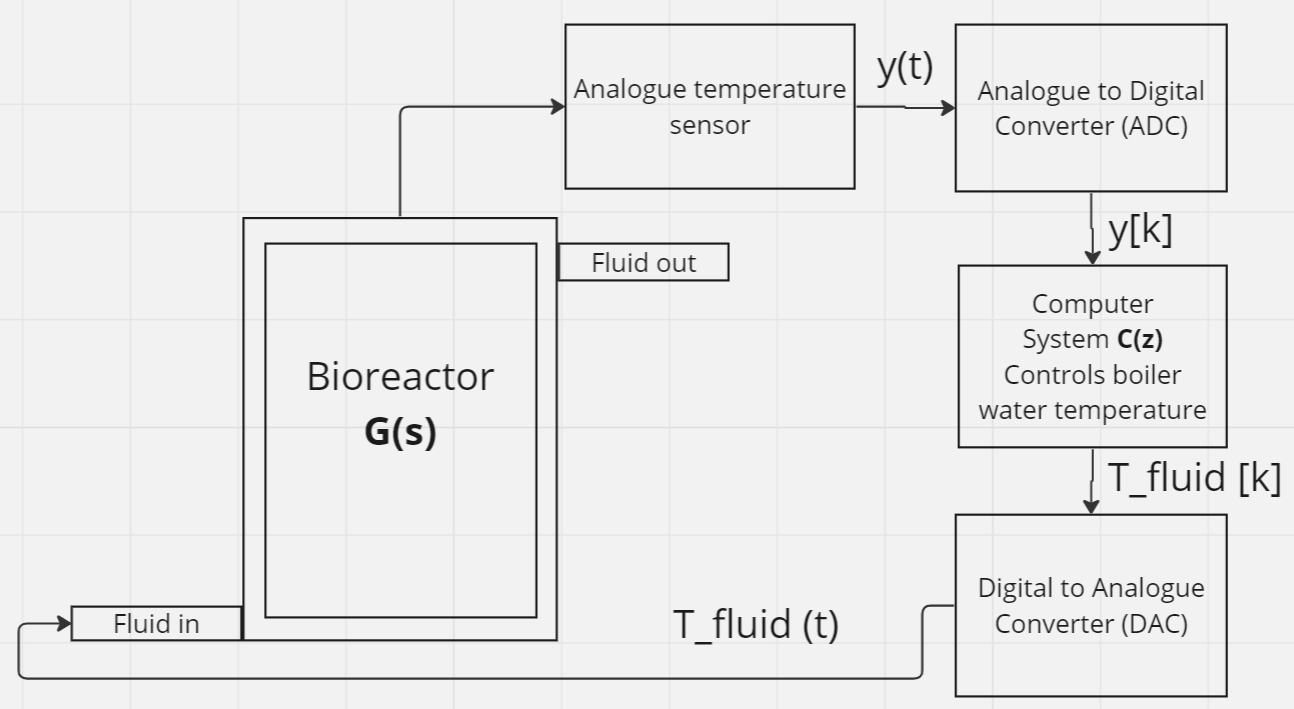
\includegraphics[width=0.6\textwidth]{eunsoo/E-1-3-digital-control-system.png}
    \hfill
    \caption{Practical implementation of the control system}
    \label{figure:E-1-3-digital-control-system}
\end{figure}

\newpage

% - (M2) the mathematical model and transfer function derivation for temperature control

The dynamics over time of temperature ($T$) can be described via the energy balance equation, where $\rho$ is the wet cell density, $V$ is the volume of the bioreactor, $c_p$ is the specific heat capacity, $Q_{met}$ is the metabolic heat generation rate, $h$ is the heat transfer coefficient and $A$ is the area of the bioreactor.

\vspace{-5mm}
\begin{equation}
    \rho V c_p \frac{\partial T}{\partial t} = Q_{met} V - hA(T-T_{fluid})
\end{equation}

The change of variables to perturbations $\Delta T = T(t) - T_{ss}$ and $\Delta T_{fluid} = T_{fluid}(t) - T_{fluid, ss}$ leads to Equation \ref{equation:E-temp-2}. During the entire culturing period ($t>0$) the steady-state assumption ($\frac{\partial \Delta T}{\partial t} = 0$, $\Delta T \approx \Delta T_{fluid} \approx 0$) can be made because otherwise the cells will die due to the violence of homeostasis. This leads to Equation \ref{equation:E-temp-3}. Substituting Equation \ref{equation:E-temp-3} into Equation \ref{equation:E-temp-2} and taking the Laplace transform leads to the desired transfer function, as shown in Equation \ref{equation:E-temp-4}.

\vspace{-5mm}
\begin{equation}
    \rho V c_p \frac{\partial \Delta T}{\partial t} = Q_{met} V - hA(T_{ss} - T_{fluid, ss}) - hA(\Delta T - \Delta T_{fluid})
    \label{equation:E-temp-2}
\end{equation}

\vspace{-10mm}
\begin{equation}
    Q_{met} V - hA(T_{ss} - T_{fluid, ss}) = 0
    \label{equation:E-temp-3}
\end{equation}

\vspace{-10mm}
\begin{equation}
    G(s) = \frac{\Delta T(s)}{\Delta T_{fluid}(s)} = \frac{hA}{\rho V c_p s + hA}
    \label{equation:E-temp-4}
\end{equation}

\subsubsection{Results}

%- (R1) the numerical values of parameters summarised in a table and justification

%- (R2) proposal of design criteria and PID controller implementation

%- (R3) demonstration of the step and impulse responses of the system and the PID controller performance

The wet cell mass of $3.5 \times 10^{-12} \ kg/cell$ and the cell diameter of $295 \times 10^{-6} \ m$ \cite{E-Furuhashi2021} are used to calculate the density so that $\rho = 0.26 \ kg/m^3$. The bioreactor height of $2 \ m$ and the bioreactor diameter of $2.1 \ m$, are used to calculate the area and the volume of the bioreactor so that $A = 20.12 \ m^2$ and $V = 6.93 \ m^3$. The yield of the final product to the wet cell $\eta = 0.5$ is used along with $c_{p, cell} = 3.440 \ kJ kg^{-1} K^{-1}$ \cite{E-Fellows2009} and $c_{p, water} = 4.180 \ kJ kg^{-1} K^{-1}$ to linearly interpolate the specific enthalpy as shown in Equation \ref{equation:E-temp-5}. The heat transfer coefficient is assumed to be $h = 0.5 \ kW m^{-2} K^{-1}$. Substituting these values in, the plant transfer function is derived as shown in Equation \ref{equation:E-temp-6}.

\vspace{-5mm}
\begin{equation}
    c_p = \eta c_{p, cell} + (1-\eta) c_{p, water} = 3.810 \ kJ kg^{-1} K^{-1}
    \label{equation:E-temp-5}
\end{equation}

\vspace{-10mm}
\begin{equation}
    G(s) = \frac{10.06}{6.872 s + 10.06}
    \label{equation:E-temp-6}
\end{equation}

The design of the controller is often done by setting the gain margin (GM) or the phase margin (PM) of $C(s)G(s)$ at a chosen frequency. The best design criterion is $PM = 60 ^{\circ}$ at $\omega = 4.16 \ rad/s$. The logic is as follows: the rise time of the plant's step response, defined as the time taken from 10\% to 90\% of the steady-state value, is $\Delta t = 1.58 - 0.07 = 1.51 \ s$, as it is also visible from Figure \ref{figure:E-1-4-step-and-impulse}. The rise time can be viewed as the mean time taken for the bioreactor to respond to the heat exchanger, and hence the period. The operating frequency is then $\omega = 2\pi / \Delta t = 4.16 \ rad/s$.

Practically, there is a higher chance of acceleration or delay in heating and cooling than a sudden overheating or underheating. Thus, one may be more concerned with the phase margin that relates to unexpected phase lags $\angle G(j \omega)$ than the gain margin that relates to unexpected magnitude deviations $|G(j \omega)|$. An acceptable rule of thumb is $PM = 60 ^{\circ}$, so one reaches the posed criterion.

One of the most commonly used controllers in the process control industry is proportional-differentiator-integral (PID). The engineer can use the above criterion along with the condition that "the low-frequency asymptote of the Nyquist on the $M=1$ line" \cite{E-Cannon2022-2}, which means the unity D.C. gain $\frac{Y(s)}{R(s)} = 1$ and thus zero steady-state error. Through this, one can find the three controller gains in $C(s) = K_p + \frac{K_i}{s} + K_d s$.

\begin{figure}[h]
    \centering
    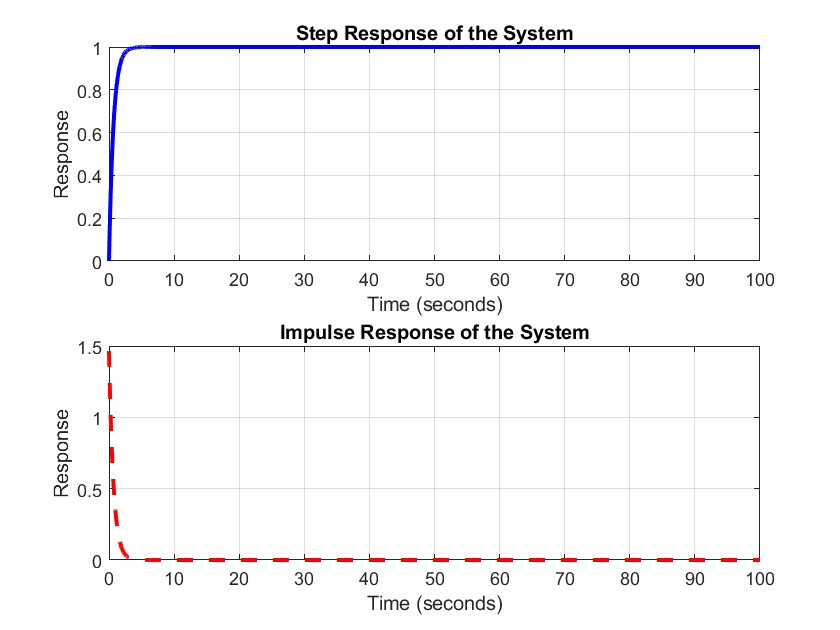
\includegraphics[width=0.7\textwidth]{eunsoo/E-1-4-step-and-impulse.jpg}
    \hfill
    \caption{The step and impulse responses of the plant}
    \label{figure:E-1-4-step-and-impulse}
\end{figure}

\vspace{-10mm}
\subsubsection{Discussion}
- (D) discussion of how my choices led to better achievement of the final objectives, compared to other control strategies

% TESTING WHERE TO PUT BIBLIOGRAPHY
% \begingroup\onehalfspacing
% {\small
% %\renewcommand{\section}[2]{}
% \begin{multicols}{2}
% \bibliographystyle{unsrt}
% %\bibliographystyle{elsarticle-num}
% % \bibliographystyle{elsarticle-harv}
% % \bibliographystyle{elsarticle-num-names}
% % \bibliographystyle{model1a-num-names}
% % \bibliographystyle{model1b-num-names}
% % \bibliographystyle{model1c-num-names}
% % \bibliographystyle{model1-num-names}
% % \bibliographystyle{model2-names}
% % \bibliographystyle{model3a-num-names}
% % \bibliographystyle{model3-num-names}
% % \bibliographystyle{model4-names}
% % \bibliographystyle{model5-names}
% % \bibliographystyle{model6-num-names}
% \bibliography{mybib.bib}
% \end{multicols}}
% \endgroup
\setlength{\headheight}{13.6pt}
\addtolength{\topmargin}{-1.6pt}
\newpage
\subsection{Oxygen control}
\setlength{\headheight}{13.6pt}
\addtolength{\topmargin}{-1.6pt}
\newpage
\subsection{Acidity control}

\setlength{\headheight}{13.6pt}
\addtolength{\topmargin}{-1.6pt}
\newpage
\section{Purification methods}
\subsection{Lactic acid purification}

\fancyhead[L]{}
\fancyhead[R]{PURIFICATION METHODS - EUNSOO CHANG}
\clearpage
\newpage
\subsection{Ammonia purification}

\setlength{\headheight}{13.6pt}
\addtolength{\topmargin}{-1.6pt}
\newpage
\section{Final product formulation}
\fancyhead[L]{}
\fancyhead[R]{FINAL PRODUCT FORMULATION - EUNSOO CHANG}
\clearpage


\newpage
\thispagestyle{nullheader}

%\begingroup\onehalfspacing
%{\small
%\renewcommand{\section}[2]{}
%\begin{multicols}{2}
%\bibliographystyle{plain}
%\bibliographystyle{elsarticle-num}
% \bibliographystyle{elsarticle-harv}
% \bibliographystyle{elsarticle-num-names}
% \bibliographystyle{model1a-num-names}
% \bibliographystyle{model1b-num-names}
% \bibliographystyle{model1c-num-names}
% \bibliographystyle{model1-num-names}
% \bibliographystyle{model2-names}
% \bibliographystyle{model3a-num-names}
% \bibliographystyle{model3-num-names}
% \bibliographystyle{model4-names}
% \bibliographystyle{model5-names}
% \bibliographystyle{model6-num-names}
%\bibliography{mybib}
%\end{multicols}}
%\endgroup
\printbibliography

\end{document}